\en
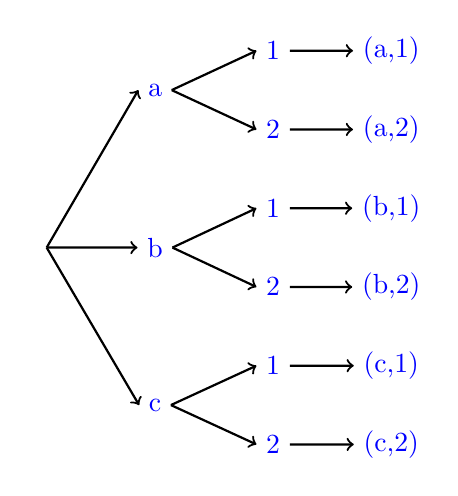
\begin{tikzpicture}
  [parent anchor=east,child anchor=west, grow=east, 
  every node/.style={circle,draw},  
  level 1/.style={sibling distance=20mm},
  level 2/.style={sibling distance=10mm},
  level 3/.style={sibling distance=10mm},
 ]
  \tikzstyle{every node}=[text=blue]
  \tikzstyle{edge from parent}=[draw, ->, solid, thick, black]
\node { }
  child {node {c} 
    child {node {2} child {node {(c,2)}} }
    child {node {1} child {node {(c,1)}} }
  }
  child {node {b} 
    child {node {2} child {node {(b,2)}} }
    child {node {1} child {node {(b,1)}} }
  }
  child {node {a}
    child {node {2} child {node {(a,2)}} }
    child {node {1} child {node {(a,1)}} }
  };
\end{tikzpicture}
\el
